\question{Câu 4}

Thiết kế mạch tính tổng 2 số sử dụng giải thuật CSA (Carry Select Adder)

Hình vẽ sau mô tả mạch tổ hợp của giải thuật CSA áp dụng cho 2 số 8 bit. Trong đó, bộ cộng 4 bit có thể chọn CLA hoặc CRA.

\begin{figure}[H]
	\centering
	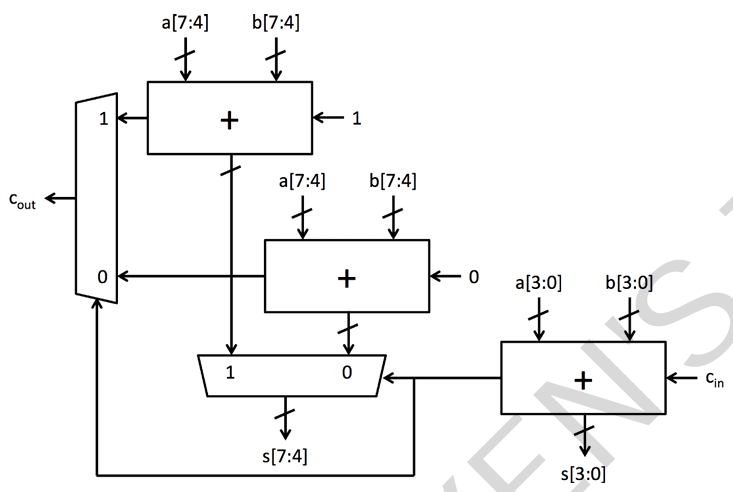
\includegraphics[width=.4\linewidth]{./my-chapters/my-images/Question4/CSA_8_bit.png}
	\caption{Bộ cộng CSA 8 bit.}
\end{figure}

Cho các standard cell là: cổng not, các cổng logic 2, 3, 4 ngõ vào, mux 2-1.

\answer{a}{Thiết kế mạch theo phương pháp đã cho và chỉ được dùng các standard cell trên.}

Bộ cộng theo kiến trúc CSA gồm một bộ cộng Full Adder 4 bit ban đầu ở đầu ghép với chuỗi các khối tính toán song song với hai giá trị ngõ vào Cin là 0 và 1, dựa vào Cout trước đó để lựa chọn kết quả và phép nhớ, từ đó giảm thời gian lan truyền phép nhớ so với kiến trúc CRA tiêu chuẩn.

Đầu tiên nhóm em sẽ thiết kế bộ cộng CRA trước, thiết kế của bộ cộng CLA đã được nhóm em trình bày ở Câu 3.
\label{key}
Khối CRA được thiết kế bằng cách ghép 4 khối Full Adder nối tiếp nhau.

\begin{figure}[H]
	\centering
	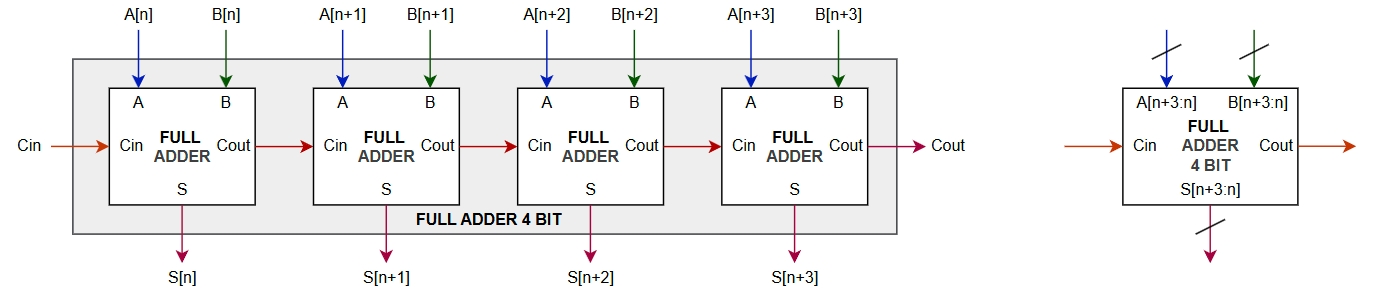
\includegraphics[width=0.9\linewidth]{./my-chapters/my-images/Question4/CRA_4_bit.png}
	\caption{Bộ cộng CRA 4 bit.}
\end{figure}

Với mỗi khối Full Adder, nhóm sử dụng thiết kế như hình:

\begin{figure}[H]
	\centering
	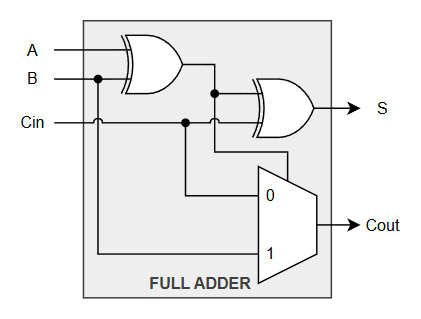
\includegraphics[width=.4\linewidth]{./my-chapters/my-images/Question4/Full_Adder.png}
	\caption{Full Adder.}
\end{figure}

Thiết kế gồm 2 cell XOR 2 ngõ vào và 1 cell MUX 2-1. Kiểu thiết kế Full Adder này sẽ sử dụng ít cell hơn (2 cell) so với kiểu thiết kế Full Adder truyền thống, đồng thời số lượng cascade giảm còn 2 giúp thiết kế hoạt động ở tốc độ cao hơn.

Tiếp theo, nhóm sẽ thiết kế khối tính toán song song.

\begin{figure}[H]
	\centering
	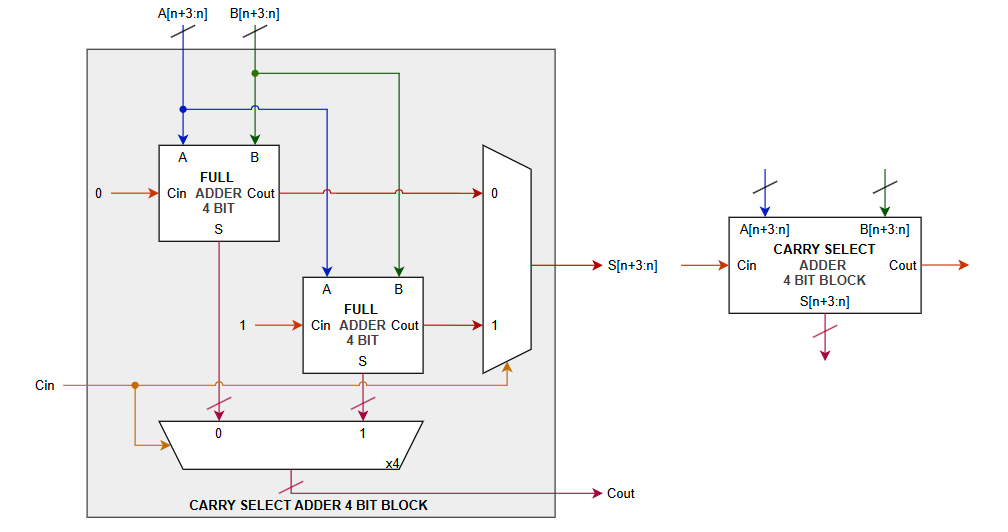
\includegraphics[width=.9\linewidth]{./my-chapters/my-images/Question4/CSA_4_bit_pair.png}
	\caption{Khối tính toán song song 4 bit.}
\end{figure}

Khối tính toán song song gồm hai bộ Full Adder 4 bit (có thể là CLA hoặc CRA) và các bộ MUX 2-1 (1 để chọn cờ nhớ và 4 để lựa chọn kết quả tính toán). 

Với yêu cầu từ đề bài, để thiết kế bộ cộng 8 bit theo giải thuật CSA, ta cần 1 bộ Full Adder 4 bit và 1 khối tính toán song song 4 bit.

\begin{figure}[H]
	\centering
	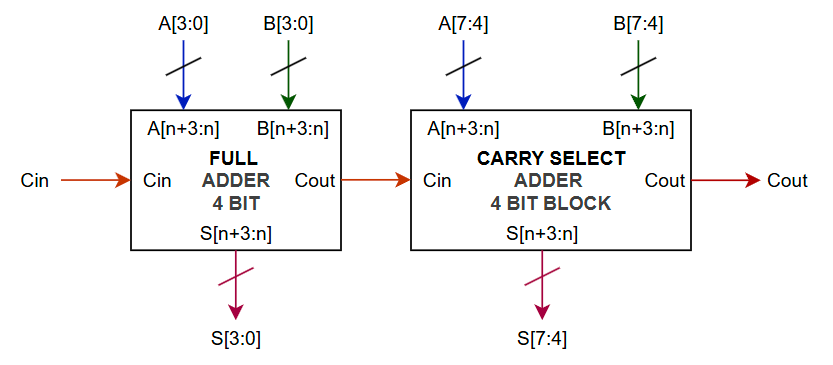
\includegraphics[width=.6\linewidth]{./my-chapters/my-images/Question4/CSA_8_bit_draw.png}
	\caption{Bộ cộng CSA 8 bit thiết kế.}
\end{figure}

Với yêu cầu mở rộng thiết kế bộ cộng 32 bit theo giải thuật CSA, ta cần 1 bộ Full Adder 4 bit và 7 khối tính toán song song 4 bit.

\begin{figure}[H]
	\centering
	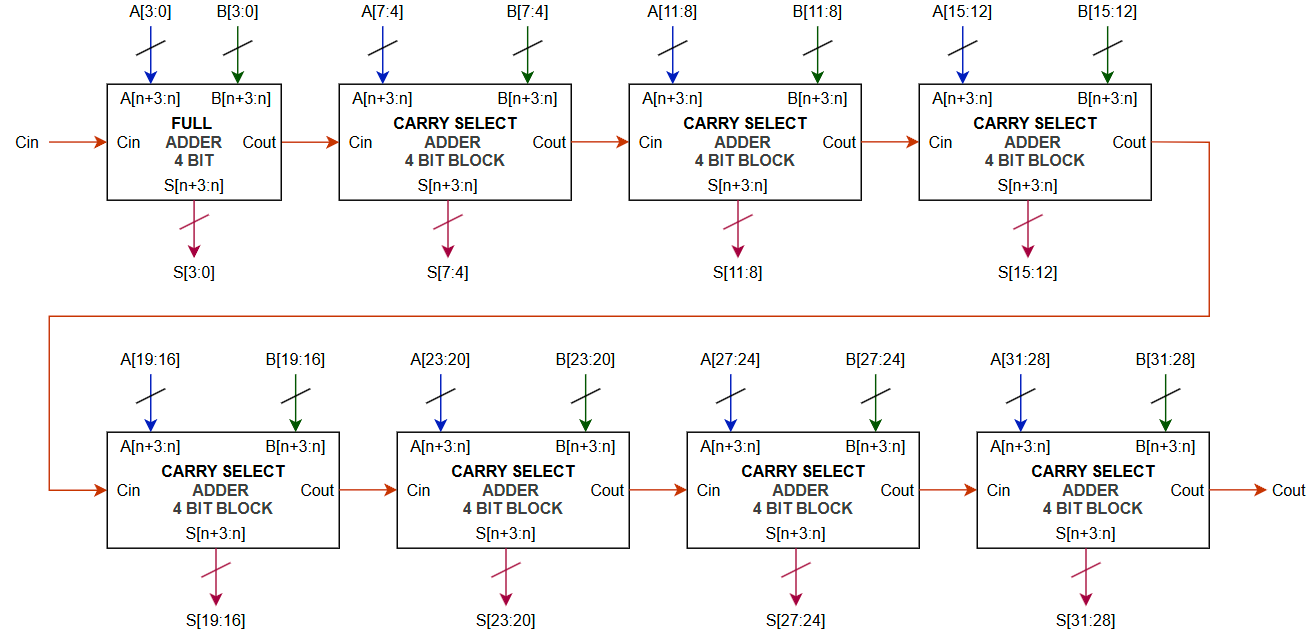
\includegraphics[width=.9\linewidth]{./my-chapters/my-images/Question4/CSA_32_bit_draw.png}
	\caption{Bộ cộng CSA 32 bit.}
\end{figure}

\answer{b}{Viết chương trình HDL mô tả mạch đã cho.}

Dựa vào yêu cầu của đề bài, nhóm cần thiết kế bộ cộng 8 bit và 32 bit bằng giải thuật, điều đó đòi hỏi HDL mô tả phải có khả năng linh hoạt (có thể điều chỉnh tham số để hình thành các thiết kế khác nhau).

\lstinputlisting[style=StyleCode, language=SystemVerilog, caption={HDL mô tả thiết kế Full Adder 1 bit.}]{./my-chapters/design_verify/Question4/fa_1b.sv}

\lstinputlisting[style=StyleCode, language=SystemVerilog, caption={HDL mô tả thiết kế CRA 4 bit.}]{./my-chapters/design_verify/Question4/cra_4b.sv}

(*) Thiết kế của khối CLA 4 bit đã được đề cập ở $\textsf{Câu 3}$.

\newpage
\lstinputlisting[style=StyleCode, language=SystemVerilog, caption={HDL mô tả thiết kế CSA linh động.}]{./my-chapters/design_verify/Question4/csa.sv}

Thiết kế gồm 2 tham số đầu vào là $\textsf{WIDTH}$ và $\textsf{CLA-CRA}$.

- $\textsf{WIDTH}$ là tham số quyết định thiết kế sinh ra phép cộng 4, 8,...,32,... bit, do đó $\textsf{WIDTH}$ luôn phải chia hết cho 4.

- $\textsf{CLA-CRA}$ là tham số quyết định bộ Full Adder 4 bit được sử dụng trong thiết kế là CLA 4 bit ($\textsf{CLA-CRA}$ >< 0) hoặc CRA 4 bit ($\textsf{CLA-CRA}$ = 0).

\answer{c}{Viết testbench cho mạch, thực hiện testbench với 100 mẫu và tính scoreboard của 100 mẫu đó.}

Phương pháp kiểm định được sử dụng tương tự với $\textsf{Câu 3}$. Kiểm thử với 100 mẫu ngẫu nhiên {a, b, Cin} được đưa vào thiết kế.

\lstinputlisting[style=StyleCode, language=SystemVerilog, caption={Kiểm định giành cho CSA.}]{./my-chapters/design_verify/Question4/csa_tb.sv}

Điểm khác biệt so với $\textsf{Câu 3}$ là testbench xuất hiện thêm tham số điều chỉnh $\textsf{WIDTH}$ nhằm để thuận tiện trong việc kiểm định hai loại thiết kế là CSA 8 bit và 32 bit. 

Vì testbench tính PASS/FAIL của kết quả và cờ nhớ riêng nên số trường hợp PASS đạt 200 so với yêu cầu là 100.

Kết quả:

\begin{lstlisting}[style=StyleResult, language=Result, caption={Kết quả kiểm định cho thiết kế CSA 8 bit.}]
	xcelium> run
	[TIME:    10] a = 0000001b, b = 0000003b, Cin = 0
	[TIME:    10] [CSA - RESULT] - PASS: Expect: 00000056, DUT: 00000056 
	[TIME:    10] [ CSA - COUT ] - PASS: Expect: 00000000, DUT: 00000000 
	
	[TIME:    20] a = 0000000e, b = 0000007a, Cin = 0
	[TIME:    20] [CSA - RESULT] - PASS: Expect: 00000088, DUT: 00000088 
	[TIME:    20] [ CSA - COUT ] - PASS: Expect: 00000000, DUT: 00000000 
	
	...
	
	[TIME:  1000] a = 0000007a, b = 00000058, Cin = 1
	[TIME:  1000] [CSA - RESULT] - PASS: Expect: 000000d3, DUT: 000000d3 
	[TIME:  1000] [ CSA - COUT ] - PASS: Expect: 00000000, DUT: 00000000 
	
	================================
	==========TEST SUMMARY==========
	Total test cases:    200    
	Passed          :    200    
	Failed          :      0    
	Pass rate       : 100.00%
	================================
	
	Simulation complete via $finish(1) at time 1010 NS + 0
	../01_tb/csa_tb.sv:62         $finish;
	xcelium> exit
\end{lstlisting}


\begin{lstlisting}[style=StyleResult, language=Result, caption={Kết quả kiểm định cho thiết kế CSA 32 bit.}]
	xcelium> run
	[TIME:    10] a = 1b4c0964, b = 3b3cd304, Cin = 0
	[TIME:    10] [CSA - RESULT] - PASS: Expect: 5688dc68, DUT: 5688dc68 
	[TIME:    10] [ CSA - COUT ] - PASS: Expect: 00000000, DUT: 00000000 
	
	[TIME:    20] a = 0e190828, b = 7a369fc6, Cin = 0
	[TIME:    20] [CSA - RESULT] - PASS: Expect: 884fa7ee, DUT: 884fa7ee 
	[TIME:    20] [ CSA - COUT ] - PASS: Expect: 00000000, DUT: 00000000 

	...
	
	[TIME:  1000] a = 7a2f41da, b = 586b58d4, Cin = 1
	[TIME:  1000] [CSA - RESULT] - PASS: Expect: d29a9aaf, DUT: d29a9aaf 
	[TIME:  1000] [ CSA - COUT ] - PASS: Expect: 00000000, DUT: 00000000 
	
	================================
	==========TEST SUMMARY==========
	Total test cases:    200   
	Passed          :    200   
	Failed          :      0  
	Pass rate       : 100.00%
	================================
	
	Simulation complete via $finish(1) at time 1010 NS + 0
	../01_tb/csa_tb.sv:61         $finish;
	xcelium> exit 
\end{lstlisting}





  

